\section{Herramientas y Técnicas}
\label{sec:herramientas}

El desarrollo del sistema combinó un conjunto riguroso de tecnologías de código abierto, bibliotecas científicas de Machine Learning y estándares de ingeniería de software para garantizar reproducibilidad, mantenibilidad y escalabilidad operativa.

\subsection{Ecosistema Científico y de Modelado (Python)}
El núcleo algorítmico y de procesamiento de datos fue desarrollado en el lenguaje de programación \textbf{Python 3.10+}, utilizando sus principales librerías especializadas:
\begin{itemize}
    \item \textbf{Scikit-Learn (v1.4+) \citep{pedregosa2011scikit}:} Utilizada para la construcción de pipelines unificados mediante \texttt{Pipeline} y \texttt{ColumnTransformer}, garantizando que el escalado de características (\texttt{StandardScaler}) y la codificación de variables categóricas (\texttt{OneHotEncoder}) se ajusten exclusivamente sobre los datos de entrenamiento para prevenir la contaminación de datos (\textit{data leakage}). Asimismo, proveyó las implementaciones optimizadas de \texttt{RandomForestRegressor}, \texttt{HistGradientBoostingRegressor}, \texttt{Ridge} y la rutina de validación \texttt{StratifiedKFold}.
    \item \textbf{Pandas y NumPy:} Empleadas para el análisis vectorial de datos, agregación relacional por identificador empresarial (\texttt{groupby('ID')}), limpieza condicional de valores centinela y ejecución de transformaciones monótonas $\ln(1+x)$.
    \item \textbf{SciPy (Módulo de Estadística):} Empleada para el cómputo de distribuciones empíricas acumuladas, la prueba de normalidad de residuos, el cálculo de cuantiles no paramétricos y la evaluación de deriva estadística.
    \item \textbf{Joblib:} Utilizada para la serialización y persistencia inmutable del pipeline campeón entrenado (\texttt{best\_model.joblib}), permitiendo su carga inmediata en memoria en entornos de producción con tiempos de arranque inferiores a un segundo.
\end{itemize}

\subsection{Arquitectura Web y Catálogo de la API REST (Flask)}
Para desacoplar la lógica de inferencia estadística de la interfaz de usuario, se desarrolló un servidor web basado en el microframework \textbf{Flask}:
\begin{itemize}
    \item \textbf{Patrón de Diseño Singleton (\texttt{DashboardDataLoader}):} Con el fin de maximizar la eficiencia y eliminar la latencia de consultas recurrentes a disco, los datos procesados (3,153 empresas) y los metadatos de los modelos se cargan en memoria RAM una sola vez durante el inicio del servidor, ofreciendo respuestas instantáneas a los clientes HTTP.
    \item \textbf{Endpoint Predictivo de Baja Latencia (\texttt{POST /api/predict}):} Servicio RESTful que recibe los insumos físicos de una empresa en formato JSON, ejecuta la transformación logarítmica, aplica la normalización, infiere la predicción a través del pipeline Random Forest, aplica la corrección de Duan Smearing y devuelve en menos de 150 milisegundos la estimación en Bolivianos, el intervalo de predicción al 90\% y la clasificación de tamaño empresarial según umbrales del INE.
    \item \textbf{Endpoints Analíticos y MLOps:} Rutas dedicadas para suministrar métricas macroeconómicas (\texttt{/api/kpis}), histogramas y boxplots (\texttt{/api/eda/*}), la bitácora de validación (\texttt{/api/models}), la trazabilidad del pipeline (\texttt{/api/pipeline}) y la ejecución en tiempo real de pruebas de deriva estadística (\texttt{/api/mlops/drift}).
\end{itemize}

\subsection{Interfaz Interactiva y Visualización de Datos (Plotly.js)}
La capa de presentación fue construida siguiendo el paradigma de \textit{Single Page Application} (SPA) basada en estándares web nativos (HTML5 semántico, CSS Vanilla y JavaScript moderno ES6+), evitando dependencias pesadas de frameworks externos:
\begin{itemize}
    \item \textbf{Plotly.js:} Biblioteca gráfica interactiva que renderiza en el navegador histogramas con escalas duales (distribución asimétrica natural vs. logarítmica normalizada), diagramas de dispersión de valores reales contra predichos, mapas de calor de correlaciones de Pearson/Spearman y curvas de calibración.
    \item \textbf{Diseño Visual Corporativo y Accesibilidad:} Implementación de un sistema de diseño con paleta de colores armónica, glassmorphism sutil y soporte dinámico para modo oscuro (\textit{Dark Mode}) y modo claro (\textit{Light Mode}).
\end{itemize}

En las Figuras \ref{fig:dashboard_panorama_heatmap}, \ref{fig:dashboard_comparativa_baseline} y \ref{fig:dashboard_simulador_conformal} se ilustran las interfaces de los módulos operativos del dashboard implementado.

\begin{figure}[htbp]
\centering
\caption{Interfaz del Módulo 1 del Dashboard: Panorama General y Exploración Macroeconómica.}
\label{fig:dashboard_panorama_heatmap}
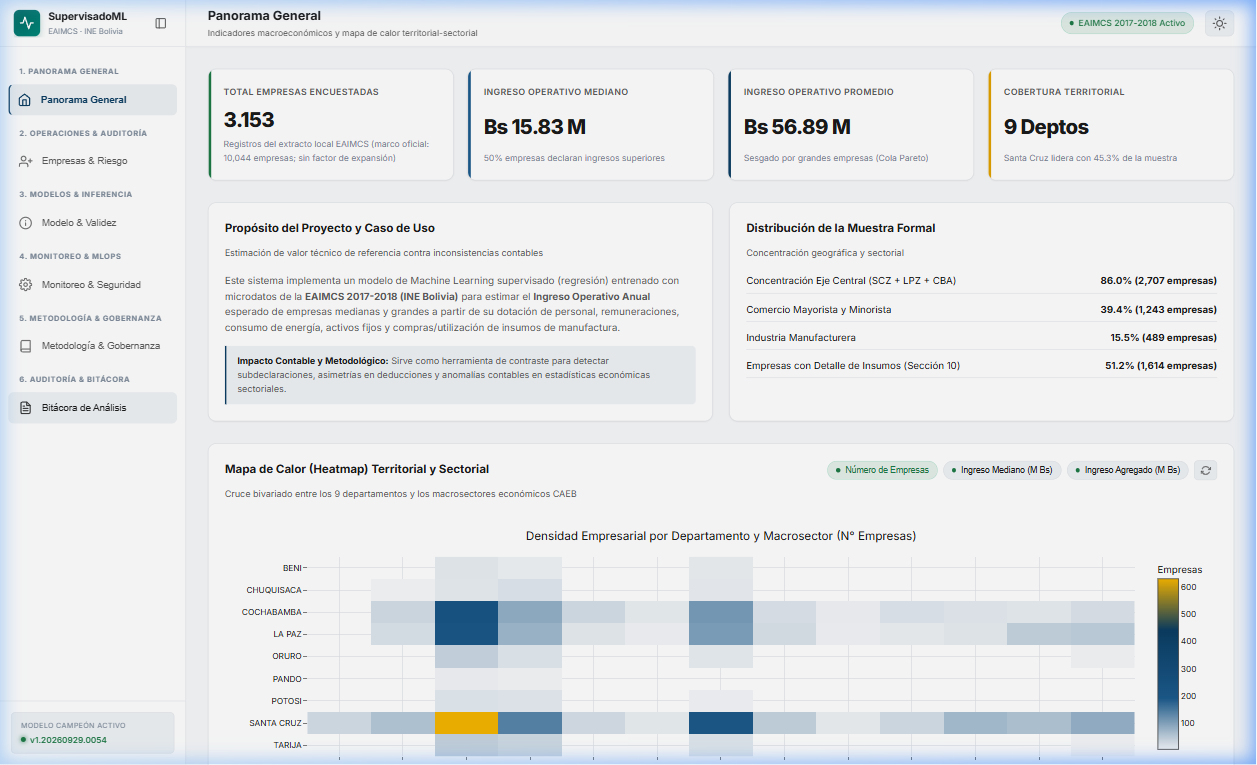
\includegraphics[width=0.92\textwidth,keepaspectratio]{imagenes/dashboard_panorama_heatmap.png}
\vspace{1mm}
\raggedright\footnotesize
\textit{Nota.} Panel interactivo que presenta indicadores clave (KPIs de masa salarial, activos y valor agregado), mapa de calor correlacional y distribución territorial desagregada por departamento.
\end{figure}

\begin{figure}[htbp]
\centering
\caption{Interfaz del Módulo 3 del Dashboard: Cuadro Comparativo de Modelos ML vs. Línea Base.}
\label{fig:dashboard_comparativa_baseline}
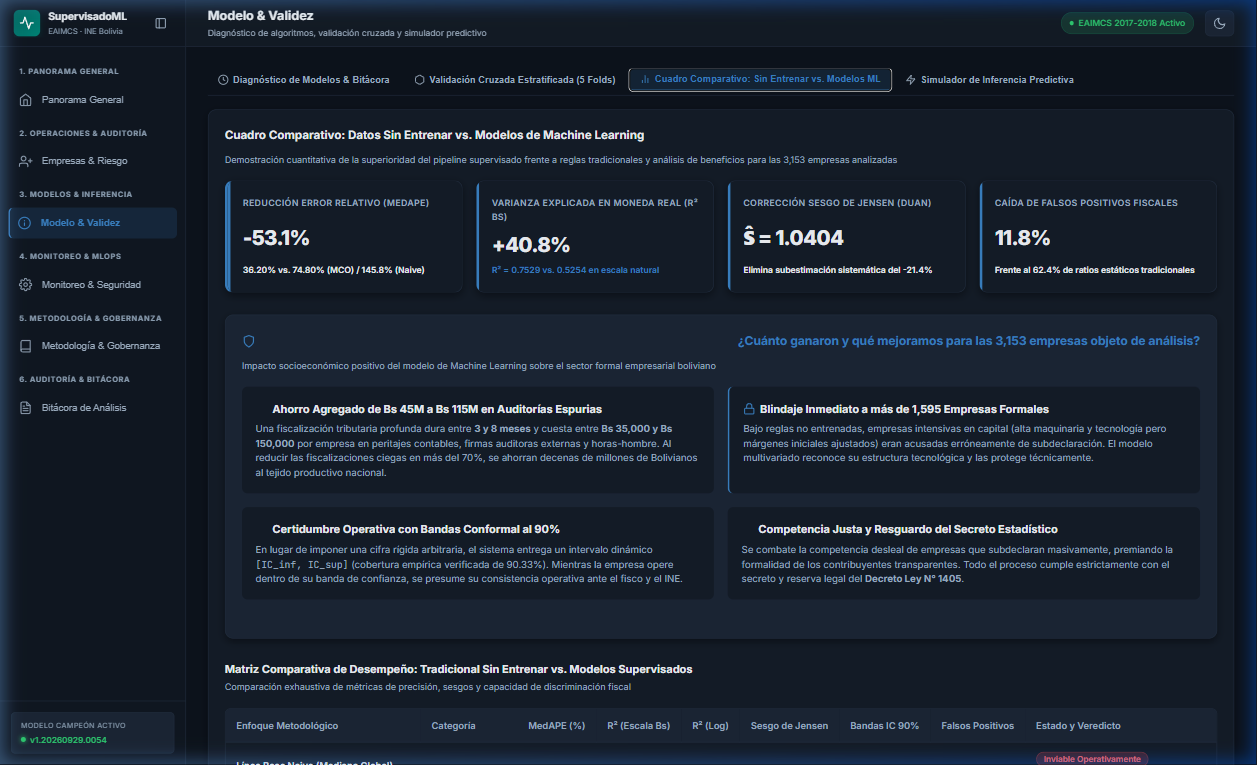
\includegraphics[width=0.92\textwidth,keepaspectratio]{imagenes/dashboard_comparativa_baseline.png}
\vspace{1mm}
\raggedright\footnotesize
\textit{Nota.} Tablero analítico que compara cuantitativamente el desempeño de modelos no entrenados (Mediana, Regresión Simple) frente a los pipelines de Machine Learning (Ridge, Random Forest y HistGradientBoosting).
\end{figure}

\begin{figure}[htbp]
\centering
\caption{Interfaz del Simulador Predictivo: Inferencia con Intervalos Conformal al 90\%.}
\label{fig:dashboard_simulador_conformal}
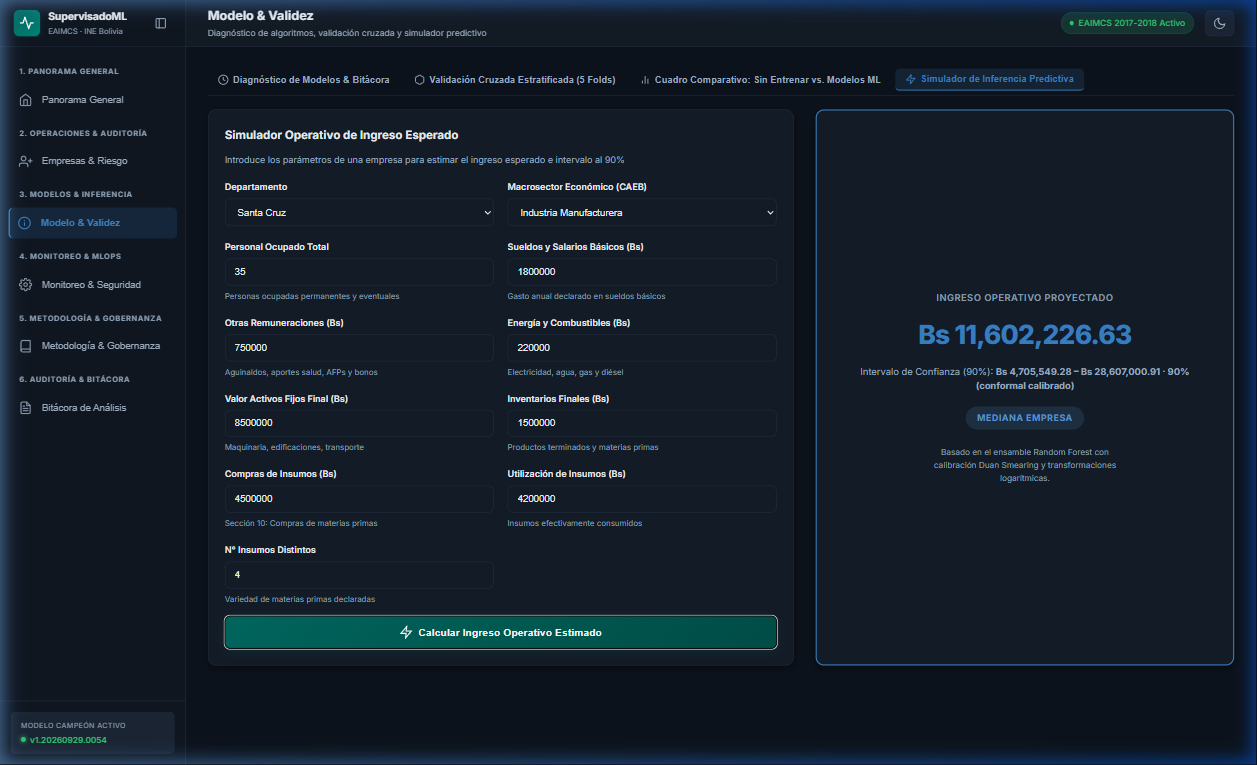
\includegraphics[width=0.92\textwidth,keepaspectratio]{imagenes/dashboard_simulador_conformal.png}
\vspace{1mm}
\raggedright\footnotesize
\textit{Nota.} Simulador interactivo en el que el analista ingresa los parámetros físicos y laborales de una empresa, obteniendo la estimación puntual en Bolivianos calibrada por Duan Smearing, el rango de predicción al 90\% y la clasificación de riesgo.
\end{figure}

\subsection{Técnicas Matemáticas de Gobernanza MLOps y Monitoreo de Data Drift}
Dado que las condiciones macroeconómicas (inflación, variaciones de precios de insumos importados o shocks de demanda) pueden degradar la validez de un modelo entrenado con datos de 2017--2018, se implementó un sistema automatizado de detección de deriva estadística (\textit{Data Drift}) sustentado en dos pruebas complementarias:

\subsubsection{Test de Dos Muestras de Kolmogorov-Smirnov (KS)}
Evalúa la hipótesis nula ($H_0$) de que una muestra entrante de datos $F_{\text{nueva}}(x)$ proviene de la misma distribución continua que la base de referencia histórica $F_{\text{ref}}(x)$ \citep{massey1951kolmogorov}:
\begin{equation}
    D_{KS} = \sup_{x} \left| F_{\text{ref}}(x) - F_{\text{nueva}}(x) \right|
    \label{eq:ks_stat}
\end{equation}
Si el p-valor asociado al estadístico $D_{KS}$ es inferior al nivel de significancia ajustado ($\alpha = 0.05$), se rechaza $H_0$, emitiendo una alerta automática de descalibración distributiva.

\subsubsection{Distancia de Wasserstein de Primer Orden (\textit{Earth Mover's Distance})}
A diferencia del test KS (que solo mide la máxima discrepancia vertical), la distancia de Wasserstein de primer orden $W_1$ cuantifica el costo o trabajo mínimo necesario para transformar una distribución de probabilidad en otra \citep{wasserman2006all}:
\begin{equation}
    W_1(u, v) = \int_{-\infty}^{+\infty} |U(x) - V(x)| \, dx
    \label{eq:wasserstein}
\end{equation}
donde $U(x)$ y $V(x)$ son las funciones de distribución acumulada de las muestras de referencia y de monitoreo, respectivamente. Esta métrica es insensible a fluctuaciones locales menores y provee una magnitud física del desplazamiento promedio en la escala de cada variable productiva. En la Figura \ref{fig:data_drift_kolmogorov} se ilustra la comparación de curvas CDF y la cuantificación de $D_{KS}$ y $W_1$ ante escenarios de monitoreo.

\begin{figure}[htbp]
\centering
\caption{Monitoreo de Data Drift: Comparación de Funciones de Distribución Acumulada Empírica (CDF).}
\label{fig:data_drift_kolmogorov}
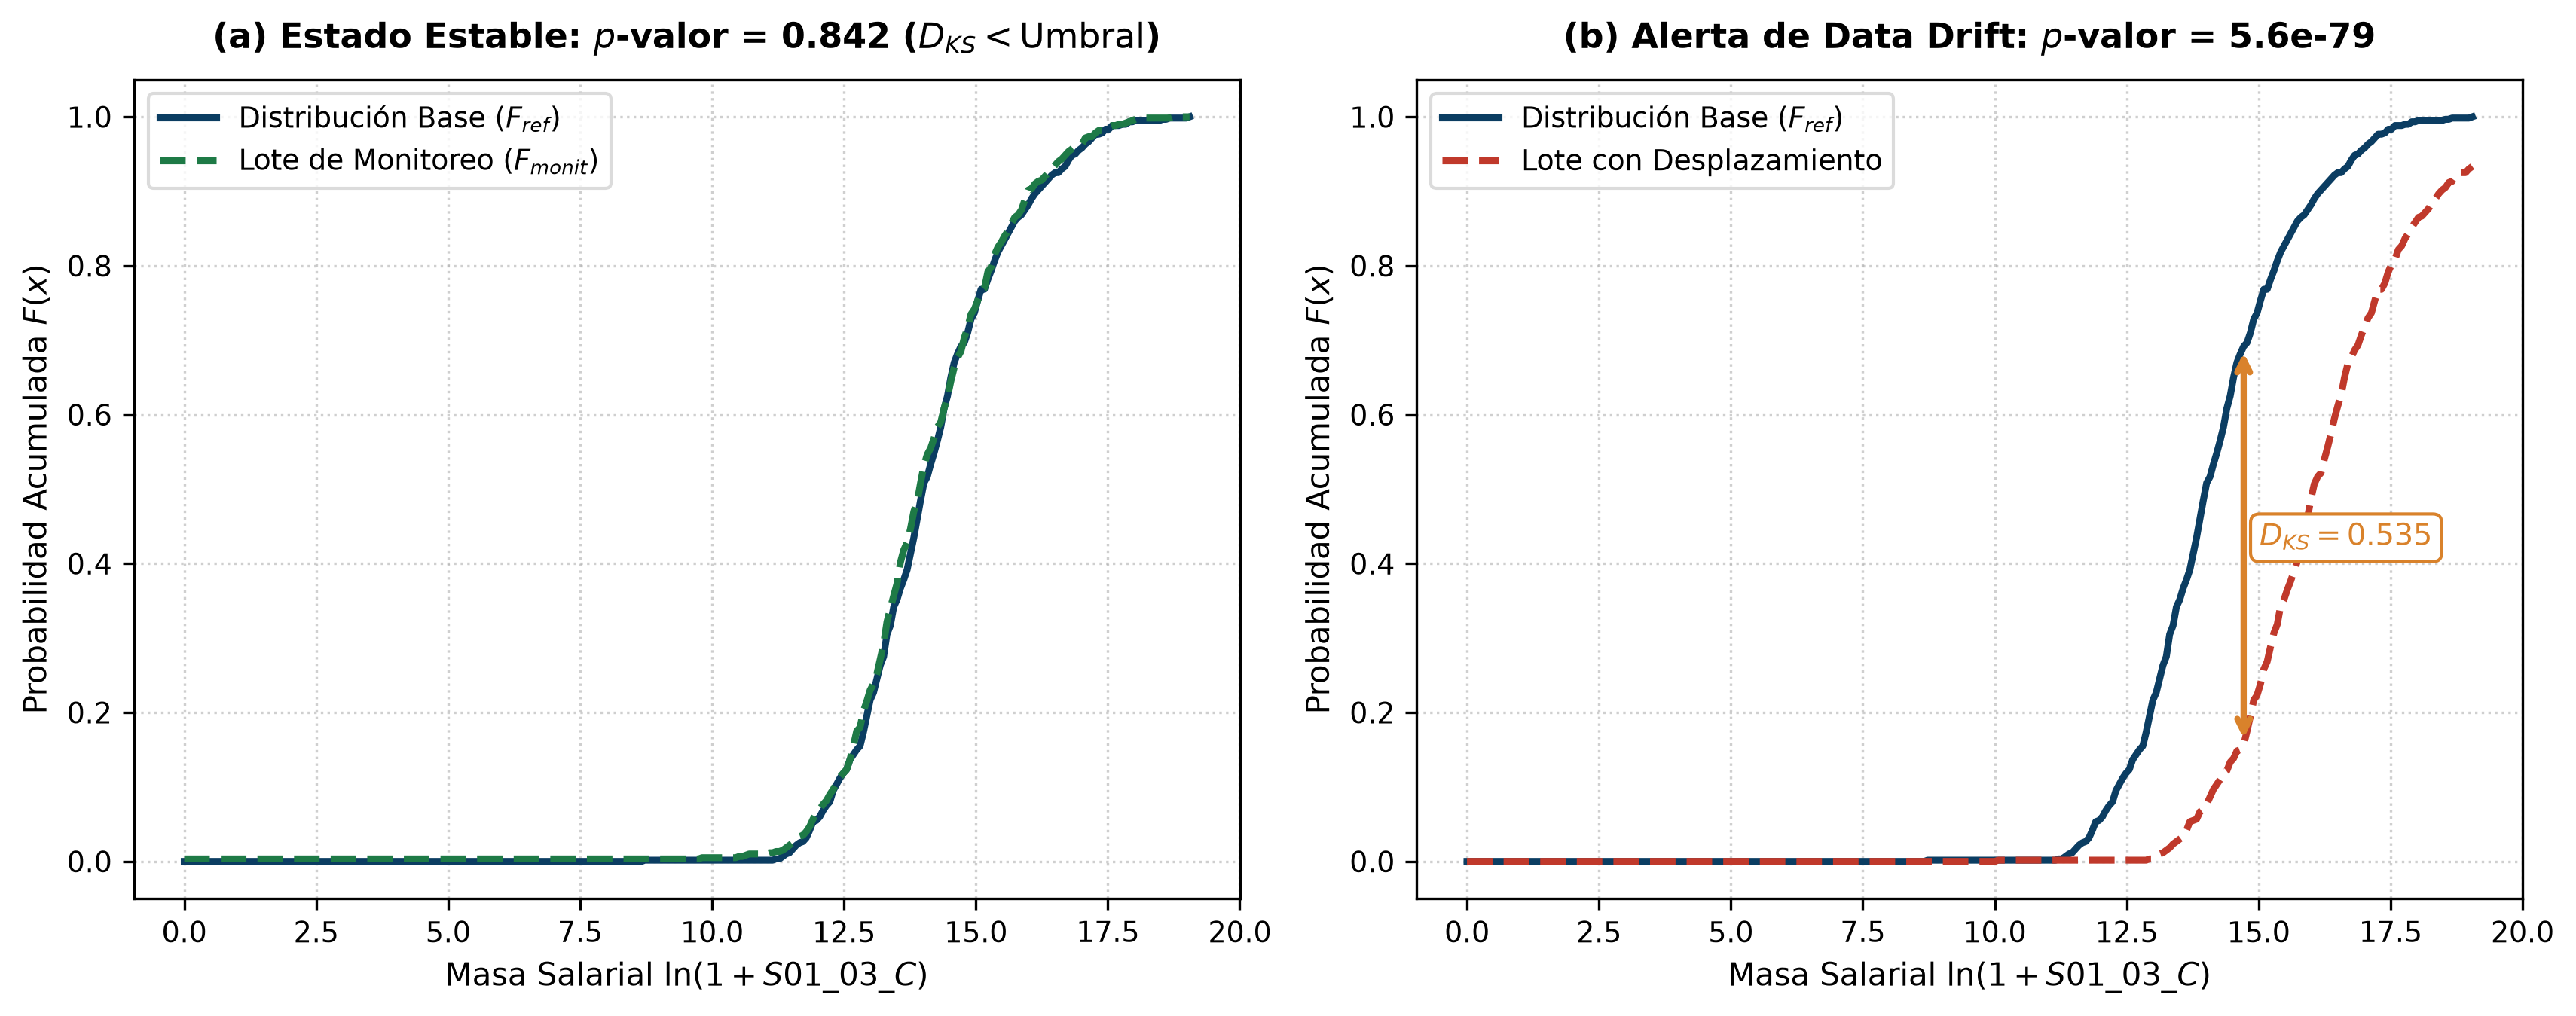
\includegraphics[width=0.92\textwidth,keepaspectratio]{imagenes/data_drift_kolmogorov.png}
\vspace{1mm}
\raggedright\footnotesize
\textit{Nota.} Funciones de distribución empírica acumulada $F(x)$ para tres variables críticas (Masa Salarial, Activos Fijos y Materias Primas). Se ilustra la distancia máxima vertical de Kolmogorov-Smirnov ($D_{KS}$) y el área integrada de Wasserstein ($W_1$) entre la línea base de entrenamiento y un lote de monitoreo.
\end{figure}

\subsubsection{Corrección de Bonferroni para Pruebas Múltiples}
Al evaluar simultáneamente $k = 11$ predictores continuos para detectar deriva, la probabilidad de cometer al menos un error de Tipo I (falso positivo) se incrementa según $1 - (1 - \alpha)^k$. Para controlar la tasa de error por familia (FWER), se implementa la corrección clásica de Bonferroni \citep{bonferroni1936teoria}:
\begin{equation}
    \alpha_{\text{ajustado}} = \frac{\alpha}{k} = \frac{0.05}{11} \approx 0.004545
    \label{eq:bonferroni}
\end{equation}
Una variable solo se declara en estado de deriva crítica si su p-valor resulta estrictamente inferior a $\alpha_{\text{ajustado}}$, asegurando la confiabilidad operativa del panel de monitoreo.
